%\noindent
\justifying
\setlength{\parskip}{1em}

%This chapter describes the methodology of the proposed image-to-image translation application, \ac{CycleGAN}(Cycle-Consistent Adversarial Network). In acp\{CycleGAN}, also, it describes the algorithm of the \ac{CycleGAN}. It explains the loss functions used to optimize the model, along with the final objective function.
%In this chapter, the methodology of the proposed image-to-image translation application. In section \ref{ProposedApproach}, the proposed approach is pictorially described and theoretically explained. In section \ref{CycleConsistentAdversarialNetworks}, the mathematics behind \ac{CycleGAN} is discussed thoroughly along with loss functions and objective functions. Also, the algorithm of the \ac{CycleGAN} described in section \ref{CycleGANAlgorithm}.

%This chapter describes the unpaired image-to-image translation method \ac{CycleGAN}. In this thesis \{CycleGAN} is used to implement image-to-image translation application.
 %and the loss functions used to optimize the model, including the final objective function. In \ac{CycleGAN}, the cycle-consistency loss function is used to unpaired image-to-image translation. The least-square loss is effective for stable learning and avoiding mode collapse, and the identity mapping loss is beneficial for preserving the color of the images after transformation. The section \ref{CycleGANAlgorithm} presents the algorithm of \ac{CycleGAN}.

%$X$ is the source domain, and $Y$ is the target domain. The domain $X$ represents synthetic data distribution, and domain $Y$ represents real data distribution. The synthetic data distribution consists of synthetic document images created using empty form templates and handwritten crops. The real data distribution consists of the real document images. 

%\section{Proposed Approach}\label{ProposedApproach}

%The proposed method for unpaired image-to-image translation is implemented using \ac{CycleGAN}.


%The final objective is achieved using three loss functions. The cycle-consistency loss to prevent the learned mappings functions $G$ and $F$ from contradicting each other. It enables \ac{CycleGAN} to learn transform images within the context\cite{zhu2020unpaired}. The least-square loss optimizes generators and discriminators\cite{mao2017squares}. The identity mapping loss to preserve the color of the input images\cite{zhu2020unpaired}.

This chapter describes the unpaired image-to-image translation method \ac{CycleGAN}. In this thesis, \ac{CycleGAN} is used to implement an image-to-image translation application. This application transforms synthetic document images into realistic document images. The application model is optimized using cycle-consistency loss, least-square loss, and identity mapping loss. These loss functions are described in this chapter. Section \ref{CycleGANAlgorithm} presents the algorithm of \ac{CycleGAN}.

\section{Cycle-Consistent Adversarial Networks}\label{CycleConsistentAdversarialNetworks}


In \ac{CycleGAN} aim is to learn the mapping function between two domains $X$ and $Y$, and vice versa. The distribution of synthetic document images represents source domain $X$ and the distribution of real document images represents target domain $Y$.  The synthetic document images created using empty form templates and handwritten crops(figure \ref{fig:InsertHandwrittenCrops}). For a given training samples $\{x_i\}_{i=1}^{N}$ where $x_i \in X$ and $\{y_j\}_{j=1}^{M}$ where $y_j \in Y$. The synthetic data distribution represented as $x \sim p_{data}(x)$ and real data distribution represented as $y \sim p_{data}(y)$. The model includes two mappings functions $G : X \rightarrow Y$ and $F : Y \rightarrow X$ as illustrated in figure \ref{fig:CycleGAN}, they are the generators. Along with generators, two adversarial discriminators $D_X$ and $D_Y$ are introduced. $D_X$ learns to distinguish images $\{x\}$ from translated images $\{F(y)\}$. In the same way, $D_Y$ learns to distinguish images $\{y\}$ from $\{G(x)\}$. Now let's try to understand the architecture of \ac{CycleGAN} using pictorial representation.

The architecture of the \ac{CycleGAN} is illustrated in figure \ref{fig:GxyFyx}. Figure (a) depicts the flow of transformation from synthetic document images to real document images. Figure (b) depicts the flow of transformation from real document images to synthetic document images. Figure \ref{fig:GxyFyx} illustrates \ac{CycleGAN} has two generators $G$ and $F$, two discriminators $D_X$ and $D_Y$. (a) The discriminator $D_Y$ takes input \textit{Input\_Y} from the target domain $Y$ and fake image \textit{Generated\_Y} generated by the generator $G$. The discriminator $D_Y$ learns to distinguish target domain images from the fake images generated by the $G$, and penalizes itself in the event of misclassification. When the discriminator $D_Y$ determines the image generated by the generator $G$ is fake. It gives feedback to generator $G$ through backpropagation to update its weights to produce good quality images. Next, to achieve cycle-consistency the fake image \textit{Generated\_Y} passed thorough generator $F$ to produce image \textit{Cyclic\_X} back in the source domain $X$, and the cycle-consistency loss is minimized between \textit{Input\_X} and \textit{Cyclic\_X}. (b) The discriminator $D_X$ takes input \textit{Input\_X} from the source domain $X$ and fake image \textit{Generated\_X} generated by the generator $F$. The discriminator $D_X$ learns to distinguish source domain images from fake images generated by the generator $F$, and penalizes itself in the event of misclassification. When the discriminator $D_X$ determines the image generated by generator $F$ is fake. It gives feedback to generator $F$ through backpropagation to update its weights to produce good quality images. Next, to achieve cycle-consistency the fake image \textit{Generated\_X} passed thorough generator $G$ to produce image \textit{Cyclic\_Y} back in the target domain $Y$, and the cycle-consistency loss is minimized between \textit{Input\_Y} and \textit{Cyclic\_Y}. The transformation flow of synthetic document images into real document images, and vice versa (marked in green dotted arrows) by minimizing the cycle-consistency loss (marked in green dotted arrows) between the input image and cyclically generated image. 

%\subsection{Formulation}

%The least-square loss\cite{mao2017squares} is used for matching the distribution of generated images to the training data distribution.
%In this thesis generators and discriminators used in \ac{CycleGAN} are optimized using least-square loss\cite{mao2017squares} which is opted from \acp{LSGAN}.
%The third is identity mapping loss to preserve the color of the input images\cite{zhu2020unpaired}.
%The general \acp{GAN} uses sigmoid cross-entropy loss function to optimize generator and discriminator. 



\begin{figure}[H]
  \centering
  \begin{minipage}[b]{1.1\textwidth}
    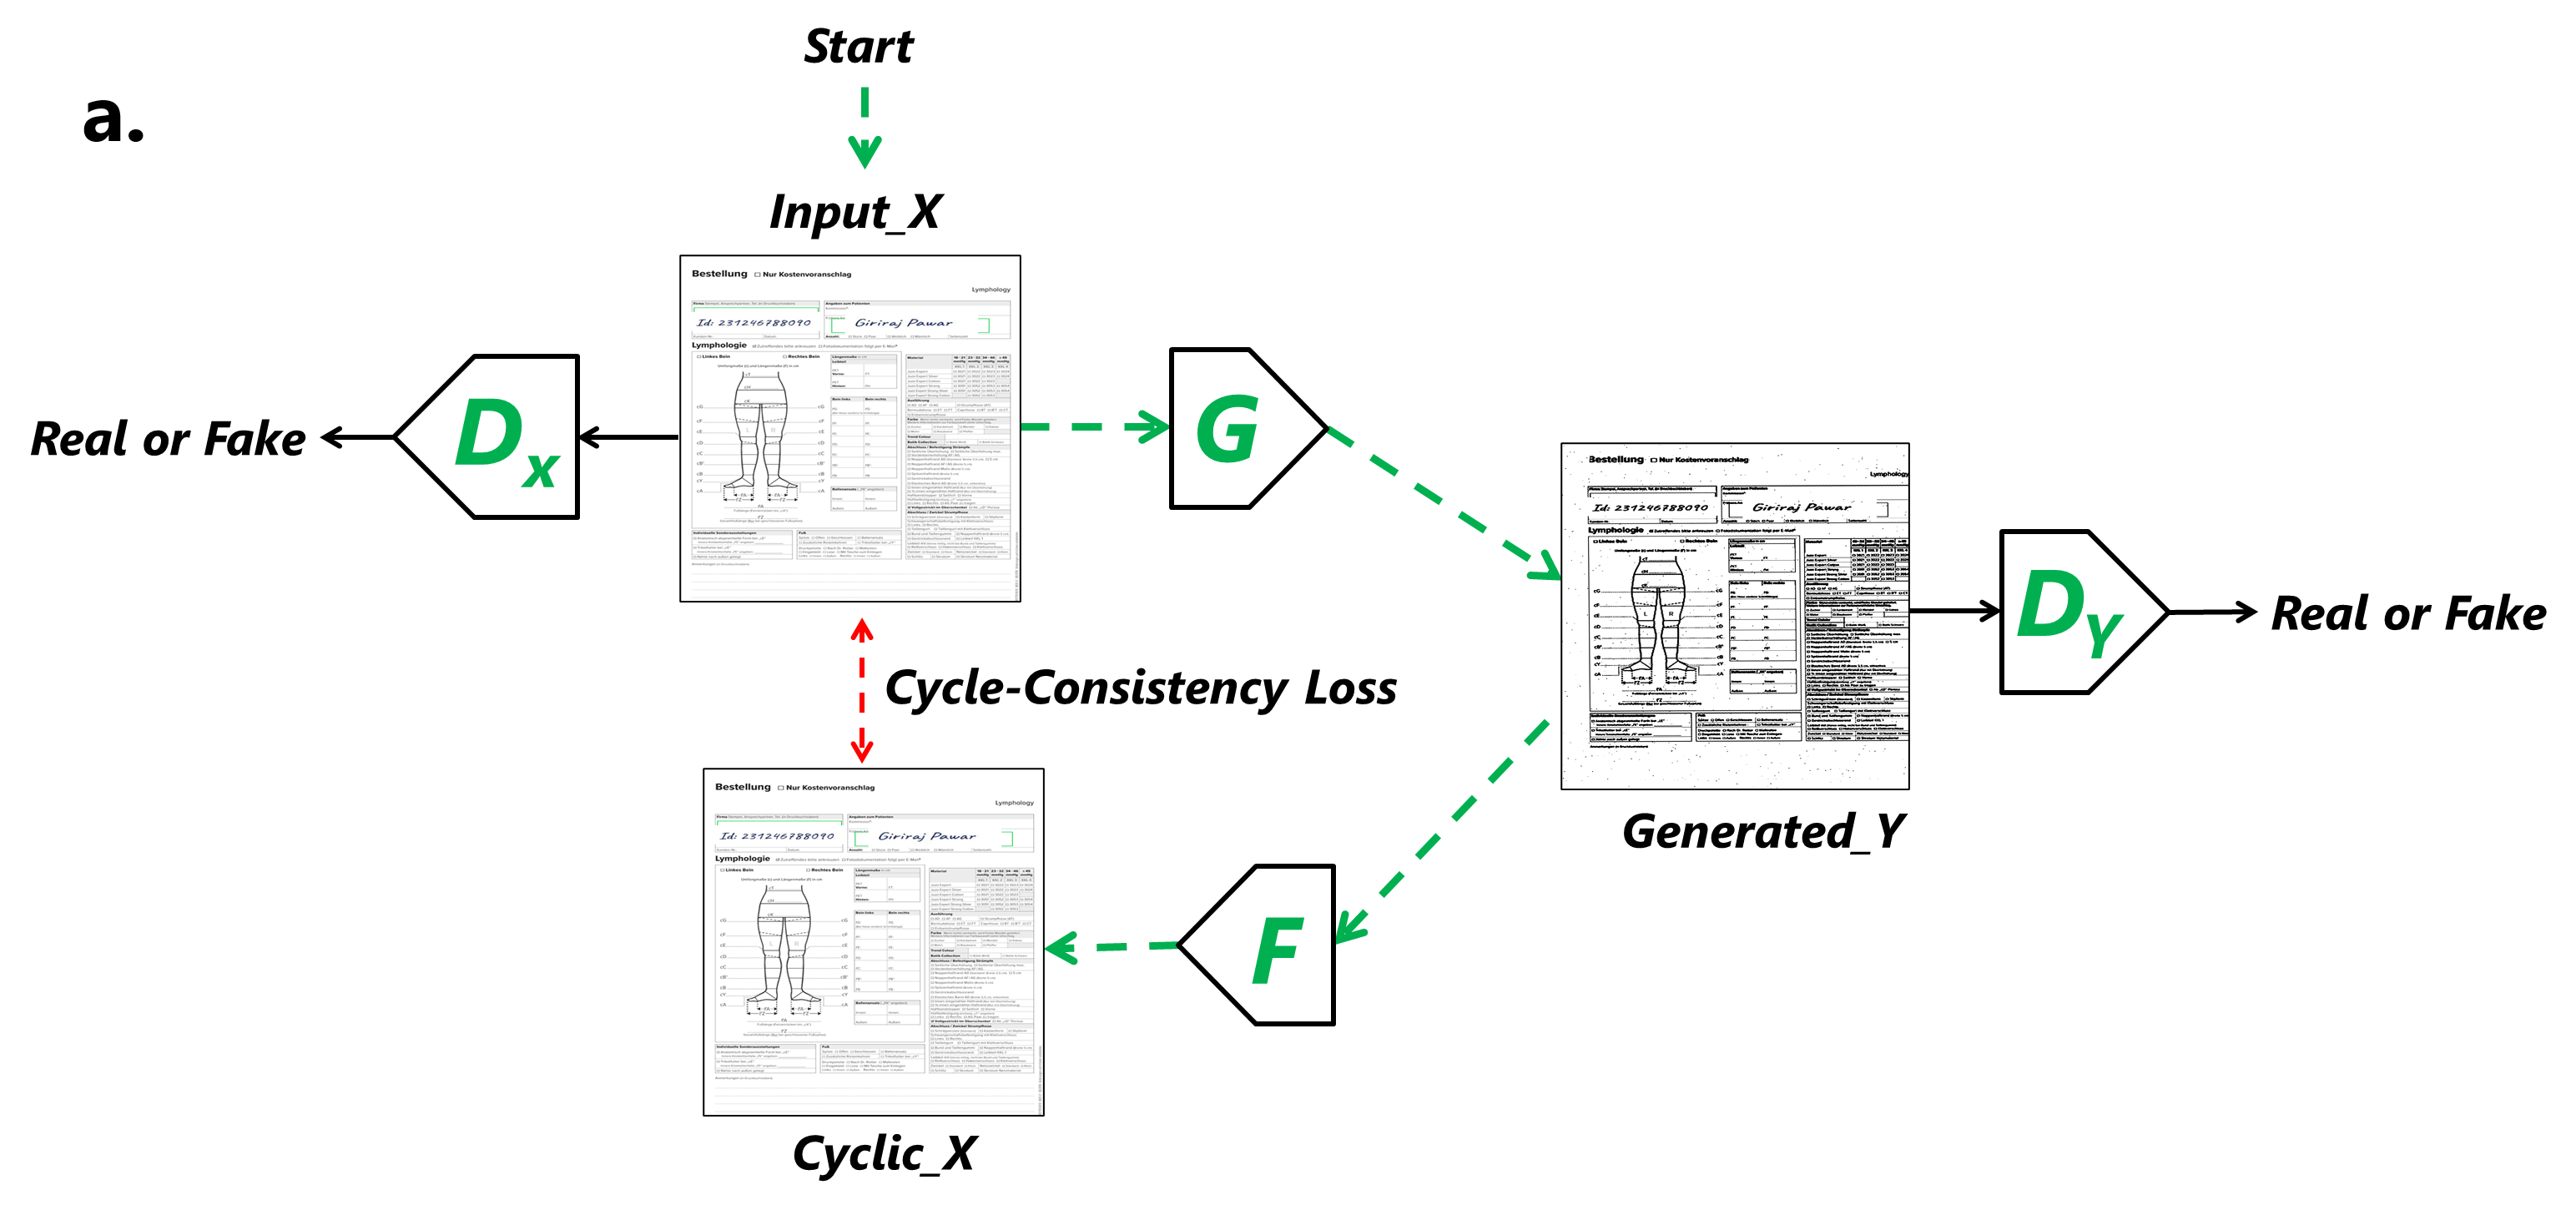
\includegraphics[width=\textwidth]{images/Methodology/Gxy.png}
  \end{minipage}
  \vfill
  \begin{minipage}[b]{1.1\textwidth}
    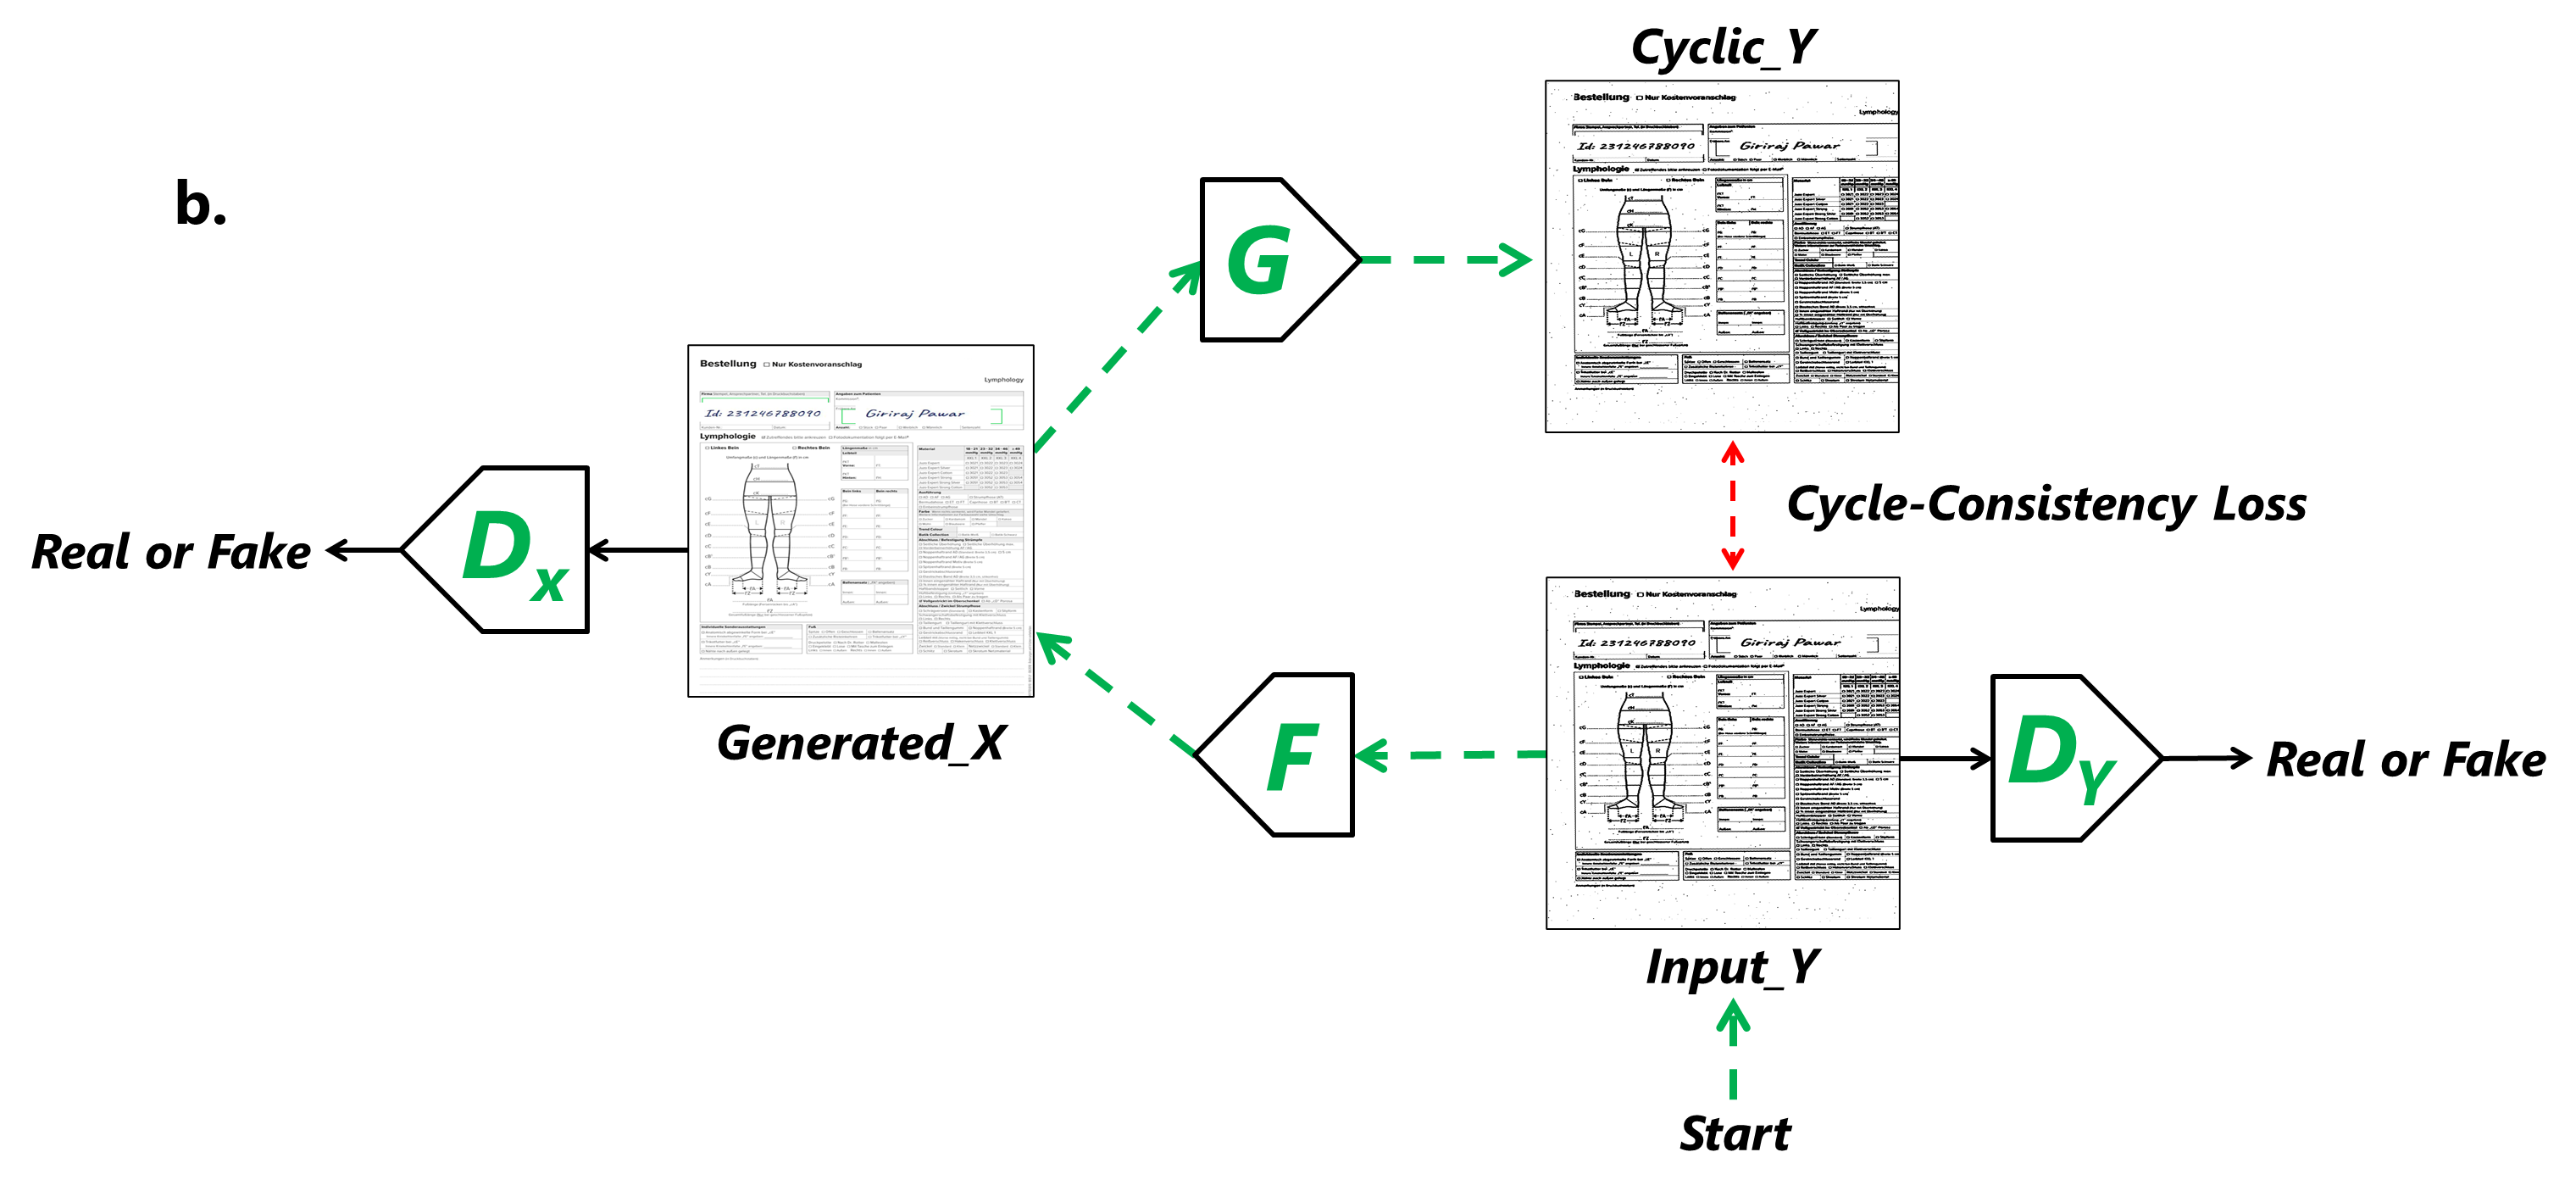
\includegraphics[width=\textwidth]{images/Methodology/Fyx.png}
  \end{minipage}
  \caption[An illustration of the proposed image-to-image translation application using \ac{CycleGAN} for transforming synthetic document images into real document images, and vice versa.]{An illustration of the proposed image-to-image translation application using \ac{CycleGAN} for transforming synthetic document images into real document images, and vice versa. It consists of two generators, $G$ and $F$ which map synthetic document images to real document images and real document images to synthetic document images, respectively minimizing cycle-consistency loss\cite{zhu2020unpaired}. It also contains two discriminators $D_X$ and $D_Y$ which acts as the adversary and reject images generated by generators.}
  \label{fig:GxyFyx}
\end{figure}

\subsection{Least-Square Loss}


In \acp{GAN} the discriminator is a binary classifier that adopts the sigmoid cross-entropy loss function. As discussed in chapter \ref{relatedworks}, while updating the generator, the sigmoid cross-entropy loss function causes the vanishing gradients problem for the samples that are on the correct side of the decision boundary but are still far from the real data.  Also, the sigmoid cross-entropy loss function causes difficulty to stabilize the model training procedure\cite{mao2017squares}. First, $\mathcal{L}_{GAN}$ (equation \ref{ganObjectiveFunction}), the negative log-likelihood objective replaced by a least-squares loss functions\cite{mao2017squares}. The least-squares loss is more stable during training and generates higher quality results\cite{mao2017squares}. It is used to optimize the generator and discriminator adversarially. In the below equations, $a$, $b$, and $c$ are the coding scheme for the equations of the discriminator. Where $a$ and $b$ are the labels for fake data and real data, respectively. $c$ denotes the value that $G$ wants $D$ to believe for fake data. Basically, $a = 0$, $b = 1$, and $c = 1$. That means fake data is represented by $0$, and real data is represented by $1$. Then the improved objective functions using least-squares loss can be defined as follows:

    \begin{equation}\label{lsgan1}
        \underset{D}{\min}\ \mathcal{L}_{ls}(D_Y) = \frac{1}{2}\ \mathbb{E}_{y \sim p_{data}(y)}\ (D_Y(y) - b)^2 + 
        \frac{1}{2}\ \mathbb{E}_{x \sim p_{data}(x)}\ (D_Y(G(x)) - a)^2
    \end{equation}
    
    \begin{equation}\label{lsgan2}
        \underset{G}{\min}\ \mathcal{L}_{ls}(G) = \mathbb{E}_{x \sim p_{data}(x)}\ (D_Y(G(x)) - c)^2]
    \end{equation}
    
    \begin{equation}\label{lsgan3}
    \mathcal{L}_{ls}(G, D_Y, X, Y) =  \underset{D}{\min}\ \mathcal{L}_{ls}(D_Y) + \underset{G}{\min}\ \mathcal{L}_{ls}(G)
    \end{equation}
    
    \begin{equation}\label{lsgan4}
        \underset{D}{\min}\ \mathcal{L}_{ls}(D_X) = \frac{1}{2}\ \mathbb{E}_{x \sim p_{data}(x)}\ (D_X(x) - b)^2 + 
        \frac{1}{2}\ \mathbb{E}_{y \sim p_{data}(y)}\ (D_X(F(y)) - a)^2
    \end{equation}
    
    \begin{equation}\label{lsgan5}        
        \underset{F}{\min}\ \mathcal{L}_{ls}(F) = \mathbb{E}_{y \sim p_{data}(y)}\ (D_X(F(y)) - c)^2
    \end{equation}
    
    
    \begin{equation}\label{lsgan6}        
        \mathcal{L}_{ls}(F, D_X, Y, X) = \underset{D}{\min}\ \mathcal{L}_{ls}(D_X) + \underset{F}{\min}\ \mathcal{L}_{ls}(F)
    \end{equation}
    

\subsection{Cycle-Consistency Loss}\label{CycleConsistencyLoss}

The cycle-consistency loss function is the basis of \ac{CycleGAN}. Theoretically, adversarial training can learn mappings that produce outputs identically distributed as target domains $Y$ and $X$, respectively\cite{goodfellow2017nips}. However, with a large amount of capacity, a neural network maps the same set of input images to any random permutations of images in the target domain,  where any of the learned mappings can produce an output distribution that matches the target distribution\cite{goodfellow2017nips}. Hence, depending just on adversarial losses alone cannot promise that the learned mapping function can map an individual input from the source domain $x_i$ to a desired output $y_j$ in the target domain. To further narrow down and reduce the space of possible outcomes using mapping functions, attempt has been made to argue that learned mapping functions should be cycle-consistent. The idea of being cycle-consistent can be understood by a simple example for translation a sentence in languages. For example, if an English sentence is translated into German and later from German to English, the outcome should be an original English sentence from where we have started. 

The figure \ref{fig:CycleGAN}, (a) \ac{CycleGAN} model with two mapping functions $G : X \rightarrow Y$ and $F : Y \rightarrow X$, and respective adversarial discriminators $D_Y$ and $D_X$ is illustrated. (b) for each image $x$ from source domain $X$, the image translation cycle should be able to bring $x$ back to the original image, i.e., $x \rightarrow G(x) \rightarrow F(G(x)) \approx x$. This is called forward cycle-consistency. (c) for each image $y$ from target domain $Y$, the image translation cycle should be able to bring $y$ back to the original image, i.e., $y \rightarrow F(y) \rightarrow G(F(y)) \approx y$. This is called backward cycle-consistency. $G$ and $F$ both should satisfy cycle-consistency. The cycle-consistency loss in the form of a mathematical equation:
%\ref{CycleConsistencyLossEquation}.

\begin{equation}\label{CycleConsistencyLossEquation}
    \mathcal{L}_{cyc}(G, F) = \mathbb{E}_{x \sim p_{data}(x)} (F(G(x)) - x) + \mathbb{E}_{y \sim p_{data}(y)} (G(F(y)) - y).
\end{equation}

\begin{figure}[H]
	    \begin{center} 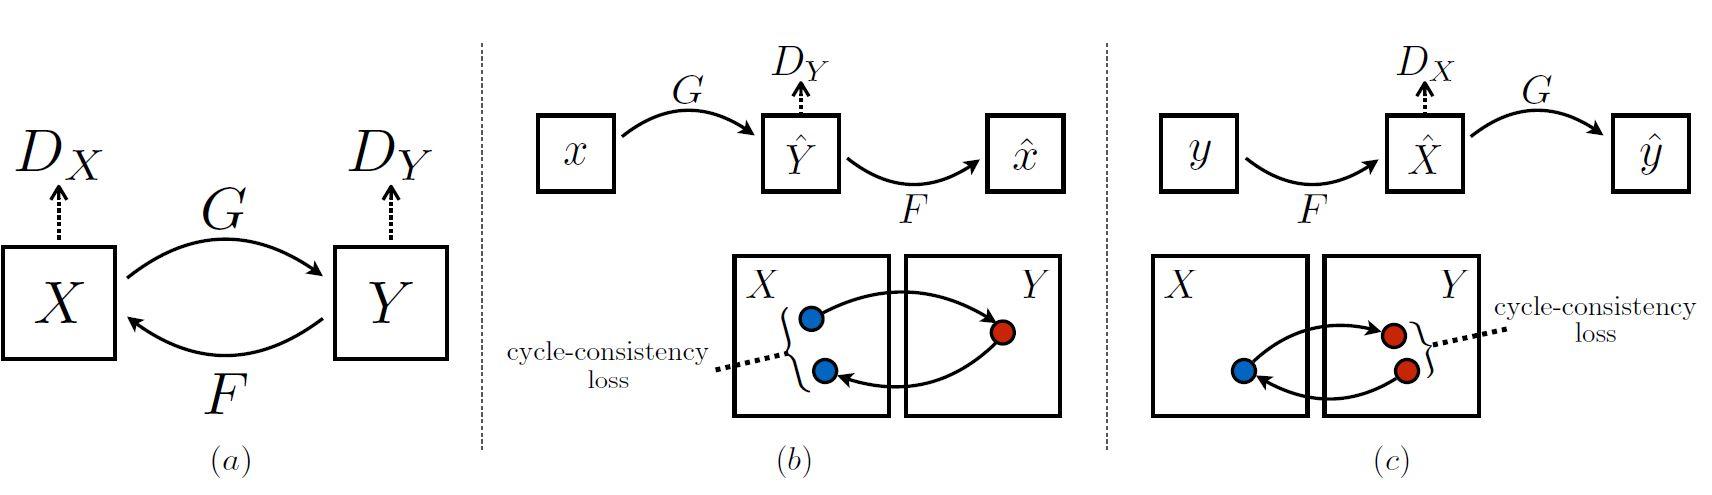
\includegraphics[scale=0.5]{images/Methodology/CycleGAN.jpg}
	    \caption[An illustration of \ac{CycleGAN} model with its mapping functions, respective discriminators, and forward and backward consistency loss.]{An illustration of \ac{CycleGAN} model with its mapping functions, respective discriminators, and forward and backward consistency loss\cite{zhu2020unpaired}.}
	    \label{fig:CycleGAN}
	    \end{center}
\end{figure}

\subsection{Identity Mapping Loss}

The identity mapping loss encourages the mapping to preserve color composition between the input and output\cite{taigman2016unsupervised}. It regularizes the generator $G$ to be near an identity mapping when real samples of the target domain are provided as the input to the generator $G$. Also, the identity mapping loss regularizes the generator $F$ to be near an identity mapping when synthetic samples of the source domain are provided as the input to the generator $F$. It means provided an input to the generator from the same domain in which it is transforming into, the output should be identical to the input. The identity mapping loss in the form of a mathematical equation:

\begin{equation}\label{IdentityMappingLoss}
    \mathcal{L}_{ide}(G, F) = \mathbb{E}_{y \sim p_{data}(y)}(F(y) - y) + \mathbb{E}_{x \sim p_{data}(x)}(G(x) - x).
    \end{equation}

\subsection{Complete Objective Function}

Combining equations \ref{lsgan6}, \ref{CycleConsistencyLossEquation}, and \ref{IdentityMappingLoss} the final objective is achieved. The model is optimized using least-squares loss, cycle-consistency loss, and identity mapping loss. In equation \ref{FullObjective}, the terms $\lambda_{cyc}$ and $\lambda_{identity}$ control the relative importance of the term in the objective. The complete objective function in the form of a mathematical equation:

\begin{equation}\label{FullObjective}
\begin{aligned}
    \mathcal{L}(G, F, D_X, D_Y) =  \mathcal{L}_{ls}(G, D_Y, X, Y)\ +\ \mathcal{L}_{ls}(F, D_X, Y, X)\ +\ 
    \lambda_{ide}\ \mathcal{L}_{ide}(G, F)\ +\ \lambda_{cyc}\ \mathcal{L}_{cyc}(G, F).
\end{aligned}
\end{equation}
    

\section{\ac{CycleGAN} Training Algorithm}\label{CycleGANAlgorithm}

%Below, the algorithm of the \ac{CycleGAN} is described in the form of pseudo-code. The pseudo-code could be understood clearly by referring to figure \ref{fig:GxyFyx}.


\begin{algorithm}[H]
\For{each training iteration}{
 \BlankLine
	Draw a random sample $x_i$ from source domain $X$ where $\{x_i\}_{i=1}^{N}$  and $x_i \in X$ \\
	\BlankLine
	Draw a random sample $y_j$ from target domain $Y$  where $\{y_j\}_{j=1}^{M}$ and $y_j \in Y$ \\
	\BlankLine
	\textbf{1. Train the Discriminators:}\\
	\BlankLine
	\BlankLine
	\Indp
		a) Compute the discriminator loss on real and fake images:\\
		\BlankLine
		\Indp
		    	$\mathcal{L}_{real,fake}^{(D_X)} = \frac{1}{2}\ (D_X(x_i) - 1)^2 + \frac{1}{2}\ (D_X(F(y_j)))^2$\\
		\BlankLine
		\BlankLine
			$\mathcal{L}_{real,fake}^{(D_Y)} = \frac{1}{2}\ (D_Y(y_j) - 1)^2 + \frac{1}{2}\ (D_Y(G(x_i)))^2$\\
		\BlankLine
		\Indm

		c) Update the discriminators\\
	\Indm
	
	\BlankLine
	\BlankLine
	\BlankLine
	
	\textbf{2. Train the Generators:}\\
	\BlankLine
	\BlankLine
	\Indp
		a) Compute the cycle-consistency losses:\\
		\BlankLine
		\Indp
			$\mathcal{L}_{cyc}^{(X \rightarrow Y \rightarrow X)} = F(G(x_i)) - x_i$\\
			\BlankLine
			$\mathcal{L}_{cyc}^{(Y \rightarrow X \rightarrow Y)} = G(F(y_j)) - y_j$\\
			\BlankLine
		\Indm
		b) Compute the identity mapping losses:\\
		\BlankLine
		\Indp
			\BlankLine	
			$\mathcal{L}_{ide}^{(X \rightarrow X)} = G(x_i) - x_i$\\
			\BlankLine
			$\mathcal{L}_{ide}^{(Y \rightarrow Y)} = F(y_j) - y_j$\\
			\BlankLine			
		\Indm
		c) Compute the Generator $G$ loss:\\
		\Indp
			\BlankLine	
			$\mathcal{L}_{G} = (D_Y(G(x_i)) - 1)^2 + \mathcal{L}_{cyc}^{(Y \rightarrow X \rightarrow Y)} + \mathcal{L}_{ide}^{(Y \rightarrow Y)}$\\
			\BlankLine	
			Compute the Generator $F$ loss:\\
			\BlankLine	
			$\mathcal{L}_{F} = (D_X(F(y_j)) - 1)^2 + \mathcal{L}_{cyc}^{(X \rightarrow Y \rightarrow X)} + \mathcal{L}_{ide}^{(X \rightarrow X)}$\\
			\BlankLine
		\Indm
		d) Update the generators\\
	\Indm	
	\BlankLine
}	


\caption{\ac{CycleGAN} training algorithm.}
\label{alg:CycleGANAlgorithm}
\end{algorithm}





















































%%%%%%%%%%%%%%%%%%%%%%%%%%%%%%%%%%%%%%%%%%%%%%%%%%%%%%%%%%%%%%%%%%%%%%%%%%%%%%%%%%%%%%%%%%%%%%%%%%%%%%%%%%%%%%%%%5

%Adversarial training can, in theory, learn mappings $G$ and $F$ that produce outputs identically distributed as target domains $Y$ and $X$ respectively. However, with large enough capacity, a network can map the same set of input images to any random permutation of images in the target domain, where any of the learned mappings can induce an output distribution that matches the target distribution. Thus, adversarial losses alone cannot guarantee that the learned function can map an individual input $x_i$ to a desired output $y_i$. To further reduce the space of possible mapping functions, we argue that the learned mapping functions should be cycle-consistent: 

%The aim is to learn mapping functions between two domains $X$ and $Y$. The Domain $X$ represents synthetic document images distribution and domain $Y$ represents real document images distribution. Given training samples $\{x_i\}_{i=1}^{N}$ where $x_i \in X$ and  $\{y_j\}_{j=1}^{M}$ where $y_j \in Y$. We denote the data distribution $x \sim p_{data}(x)$  and $y \sim p_{data}(y)$.

\begin{comment}
\subsection{Adversarial Loss}
We apply adversarial losses\cite{goodfellow2014generative} to both mapping functions. For the mapping function $G : X \rightarrow Y$  and its discriminator $D_Y$ , we express the objective as:

    \begin{equation}\label{AdversarialLoss}
    \mathcal{L}_{GAN}(G, D_Y, X, Y) = \mathbb{E}_{y \sim p_{data}(y)} [\log D_Y(y)] + \mathbb{E}_{x \sim p_{data}(x)}[\log (1 - D_Y(G(x)))],
    \end{equation}
    
where $G$ tries to generate images $G(x)$ that look similar to images from domain $Y$ , while $D_Y$ aims to distinguish between translated samples $G(x)$ and real samples $y$. $G$ aims to minimize this objective against an adversary $D$ that tries
to maximize it, i.e., $\min_{G} \max_{D_Y} \mathcal{L}_{GAN}(G, D_Y, X, Y)$. We introduce a similar adversarial loss for the mapping function $F : Y \rightarrow X$ and its discriminator $D_X$ as well: i.e., $\min_{F} \max_{D_X} \mathcal{L}_{GAN}(F, D_X, Y, X)$.

\end{comment}

\begin{comment}
We aim to solve:
\begin{equation}\label{FullObjectiveAimToSolve}
    G^*, F^* = \arg\underset{G, F}{\min}\underset{D_X, D_Y}{\min} \mathcal{L}(G, F, D_X, D_Y)
    \end{equation}
\end{comment}


\begin{comment}
\begin{figure}[H]
        \begin{center}
    	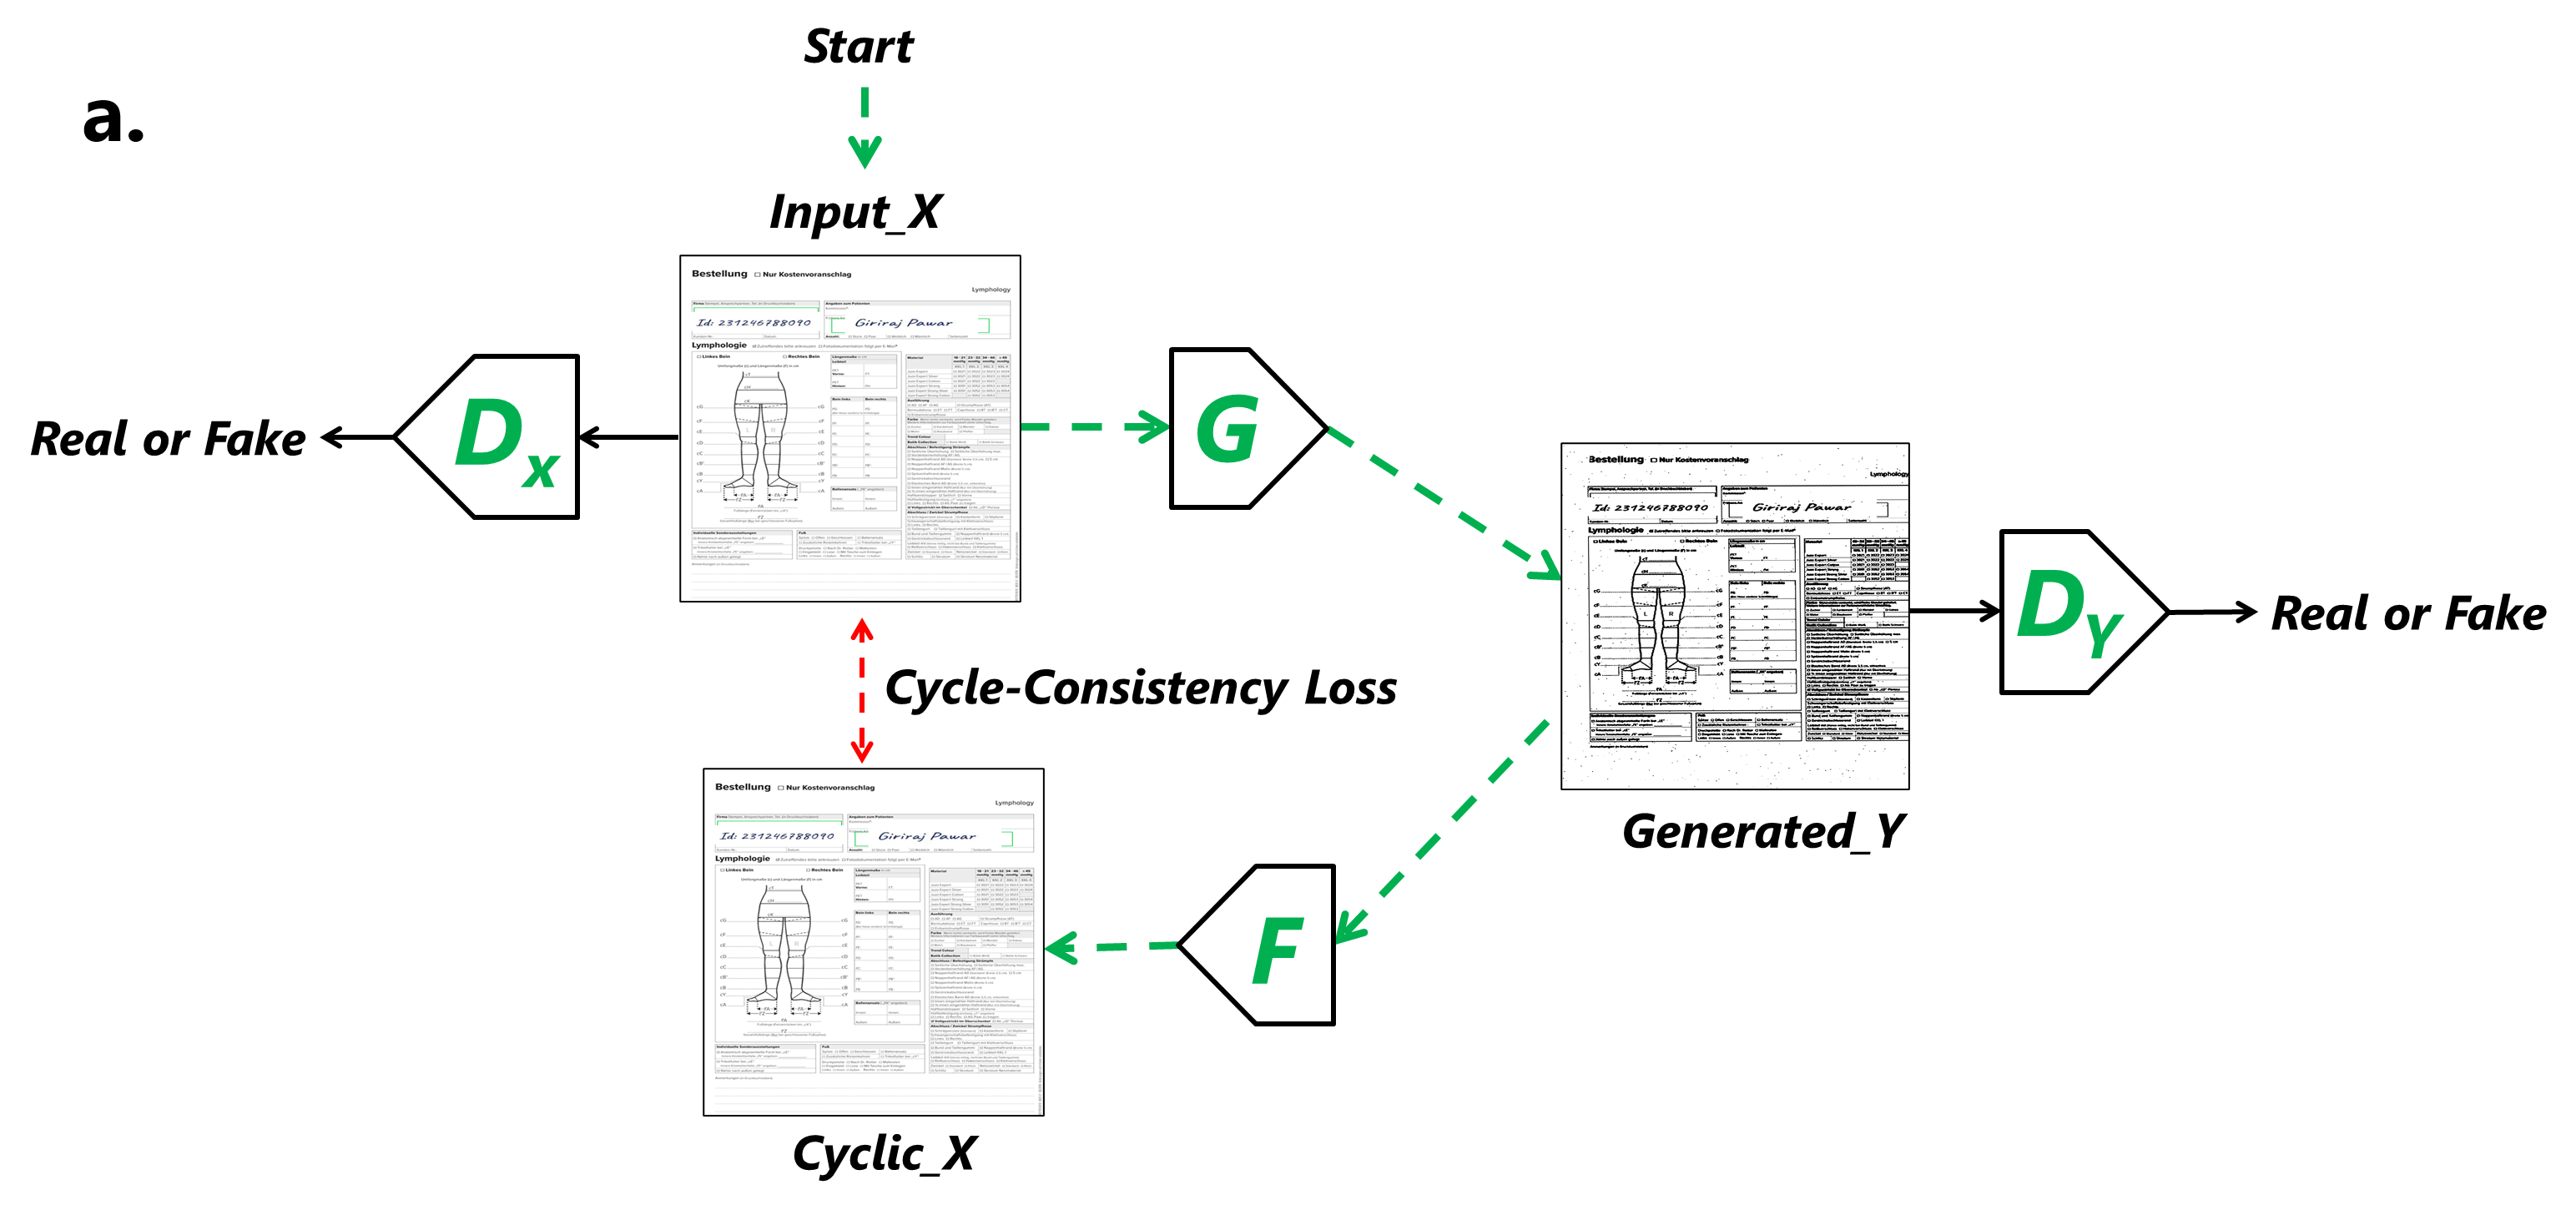
\includegraphics[scale=0.20]{images/Methodology/Gxy.png}
	    \caption[The transformation flow of synthetic document images into realistic document images using generator $G$.]{The transformation flow of synthetic document images into realistic document images using generator $G$. The transformation flow is marked by green dotted arrows. The generator $G$ is a mapping function $G: X \rightarrow Y$ which transforms images from the source domain to the target domain by minimizing the cycle-consistency loss (red dotted arrow) between the input image and cyclically generated image.}
	    \label{fig:Gxy}
	    \end{center}
\end{figure}

\begin{figure}[H]
        \begin{center}
    	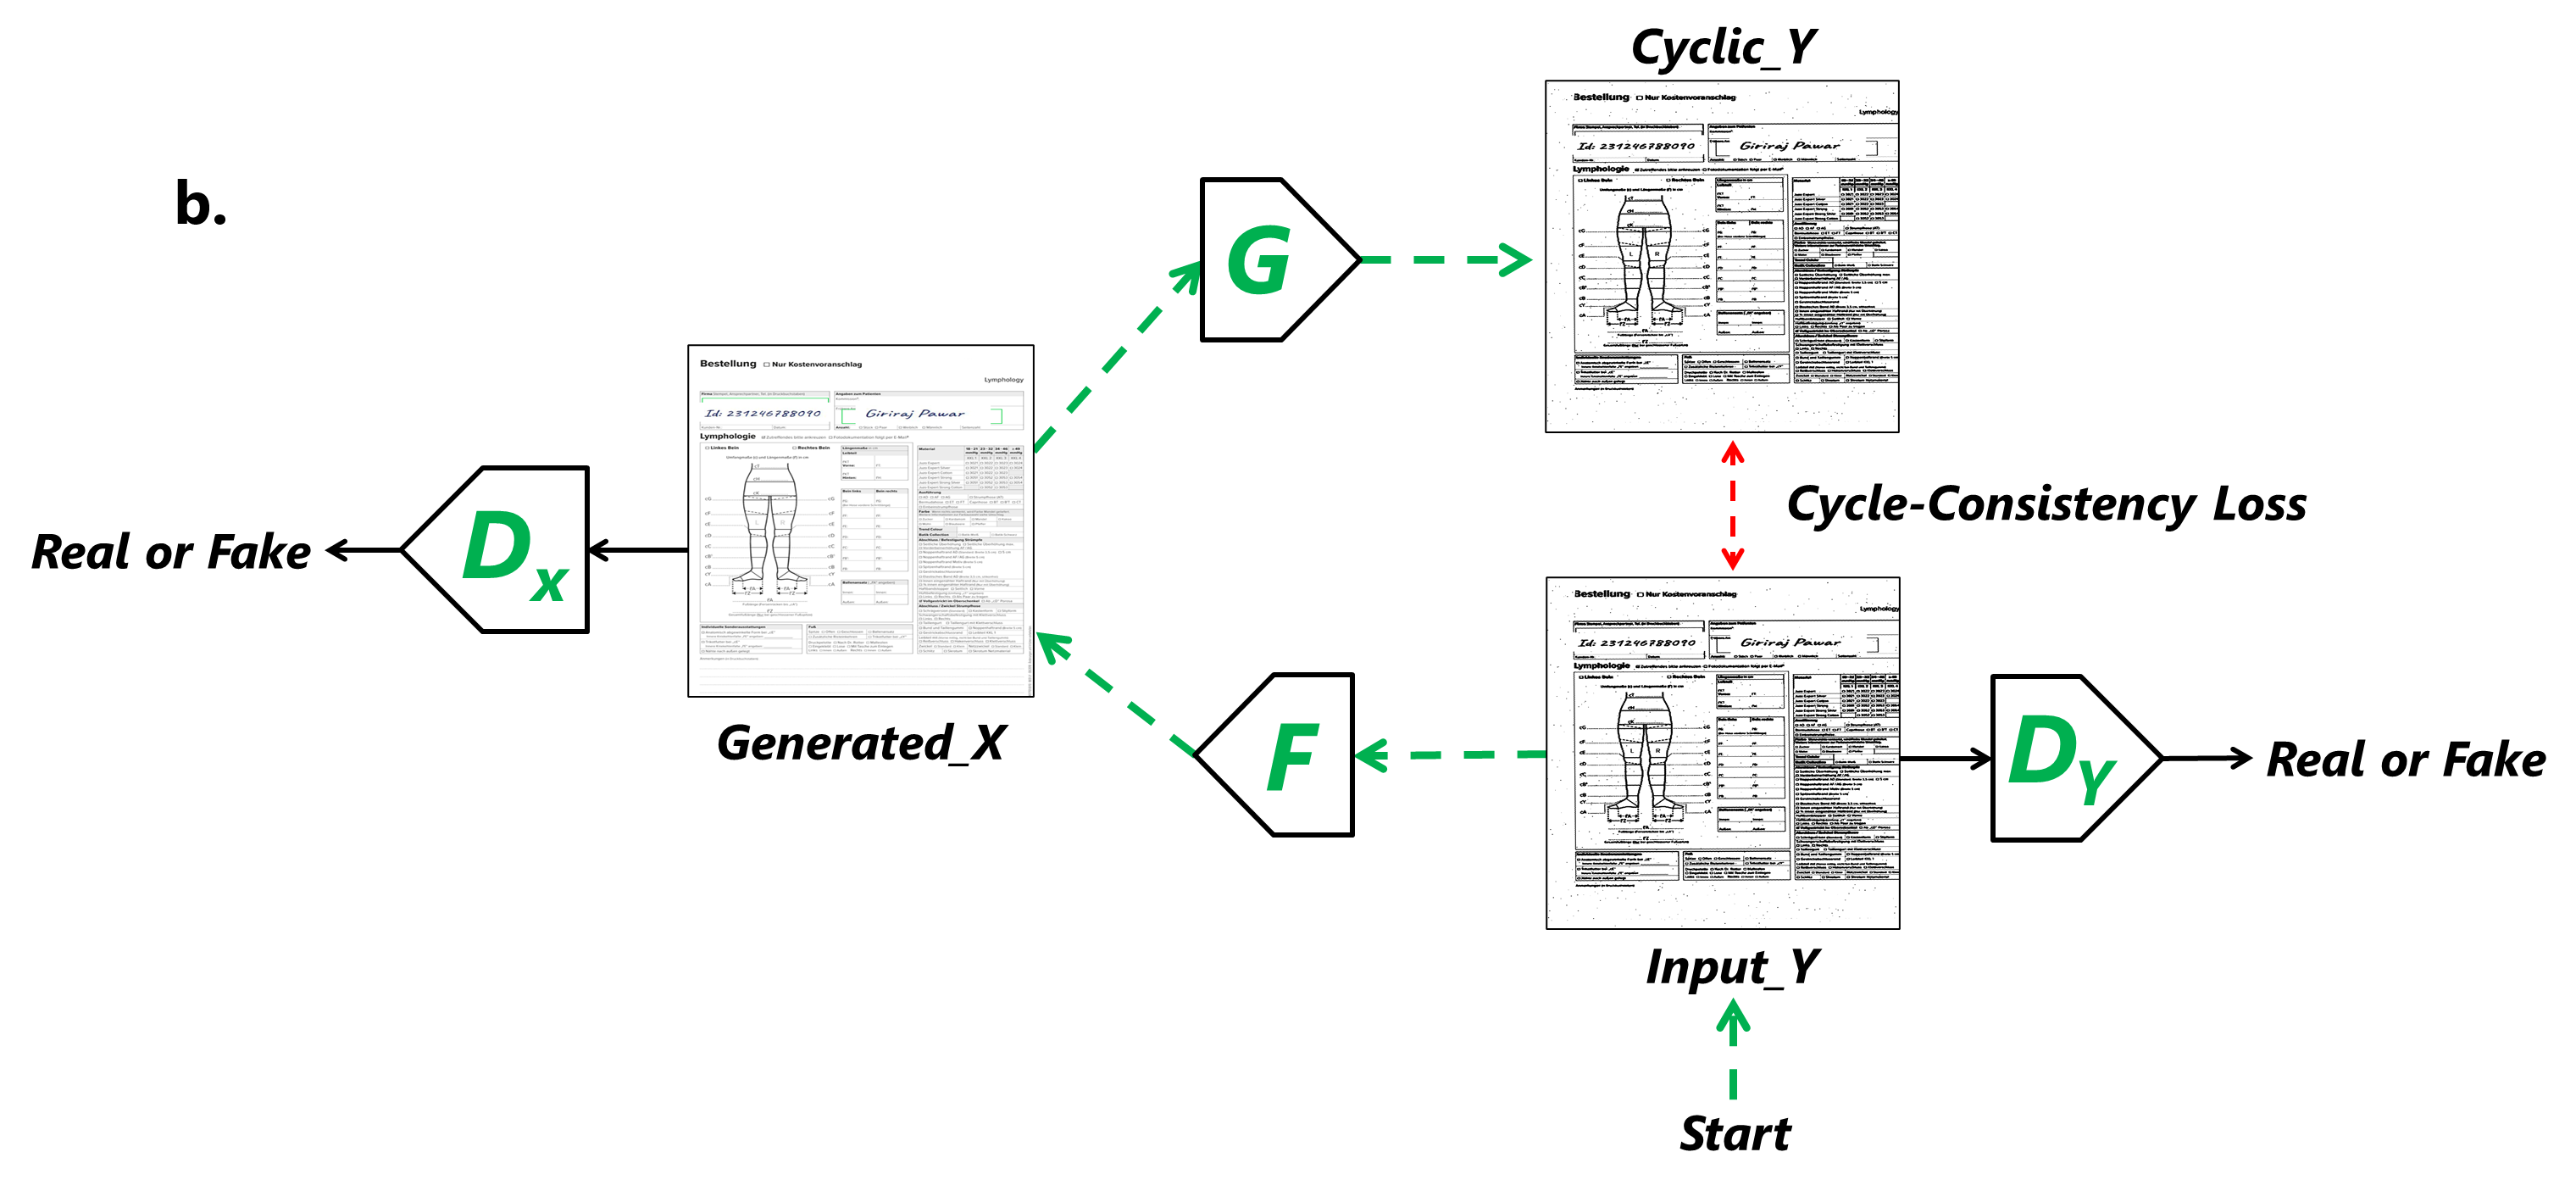
\includegraphics[scale=0.20]{images/Methodology/Fyx.png}
	    \caption[The transformation flow of real document images into synthetic document images using generator $F$.]{The transformation flow of real document images into synthetic document images using generator $F$. The transformation flow is marked in green dotted arrows. The generator $F$ is mapping function $F: Y \rightarrow X$ which transforms images from the target domain to the source domain by minimizing the cycle-consistency loss (red dotted arrow) between the input image and cyclically generated image.}
	    \label{fig:Fyx}
	    \end{center}
\end{figure}


%It is helpful to introduce an additional loss to encourage the mapping to preserve color composition between the input and output. In particular, we adopt the technique of\cite{taigman2016unsupervised} and regularize the generator to be near an identity mapping when real samples of the target domain are provided as the input to the generator

%Below, the algorithm of the \ac{CycleGAN} is described in the form of pseudo-code. The pseudo-code could be understood clearly by referring to figure \ref{fig:GxyFyx}.



\begin{algorithm}[H][1]
\For{each training iteration}{
 \BlankLine
 \BlankLine
 \BlankLine
 \textbf{1. Train the Generators:}
	\BlankLine
	\BlankLine
	\Indp
	1. Get a random image \textit{Input\_X} from source domain $X$ from the training dataset.\\
	2. Get a random image \textit{Input\_Y} from target domain $Y$ from the training dataset. \\
	\BlankLine
 	\BlankLine
	3. Pass \textit{Input\_X} through generator $G$ and generate fake image \textit{Generated\_Y}.\\
	4. Pass \textit{Input\_Y} through generator $F$ and generate fake image \textit{Generated\_X}.\\
	\BlankLine
 	\BlankLine
	5. Pass \textit{Generated\_Y} through generator $F$ and generate cyclic image \textit{Cyclic\_X}.\\
	6. Pass \textit{Generated\_X} through generator $G$ and generate cyclic image\textit{Cyclic\_Y}.\\
	\BlankLine
 	\BlankLine
	7. Pass \textit{Input\_X} through generator $G$ and generate identical image \textit{Same\_X}.\\
	8. Pass \textit{Input\_Y} through generator $F$ and generate identical image \textit{Same\_Y}.\\
	\BlankLine
 	\BlankLine
 \Indm
 \textbf{2. Train the Discriminators:}
	1. Pass \textit{Input\_X} through generator $G$ and generate identical image \textit{Same\_X}.\\
     2. Pass \textit{Input\_Y} through generator $F$ and generate identical image \textit{Same\_Y}.\\
 	\BlankLine
 	\BlankLine
	\Indp
	
\BlankLine
\BlankLine
\BlankLine
}	
	\caption{CycleGAN training algorithm.}
\label{alg:CycleGANAlgorithm}
\end{algorithm}





\end{comment}

